\section{Evaluation}
\label{sec:evaluation}

Our evaluation is structured around seven research questions, each pinned to a specific subset of the artifact registry. We use the consolidated tables produced by the paper-artifact pipeline. We do not introduce new experiments here; we report the artifacts as they exist.

\subsection{RQ1: Does masked execution preserve correctness across model components and architectures?}
\label{sec:eval:rq1}
\paragraph{Setup.}
We run the masked wrapper against a plain reference on (i)~GPT-2 model-level wrapper (\texttt{sshleifer/tiny-gpt2}), including full forward, prefill, decode-step, and greedy generation; (ii)~modern decoder-only block wrapper (RMSNorm + SwiGLU + RoPE + GQA), synthetic and tiny-HF configurations; (iii)~modern decoder-only model wrapper, prefill + decode-step + greedy generation; and (iv)~compatible nonlinear islands across decoder-only, encoder-only, encoder-decoder, and modern-decoder architectures.

\paragraph{Metric.} \texttt{allclose} against the plain reference; per-component $\max|\!\cdot\!|$ error.

\paragraph{Result.}
The GPT-2 and modern-decoder model wrappers reproduce the plain reference output token-for-token in the tested configurations. \Cref{tab:correctness-summary} lists $19$ component rows; \Cref{fig:correctness-error-summary} plots the per-component errors.

\begin{figure}[h]
\centering
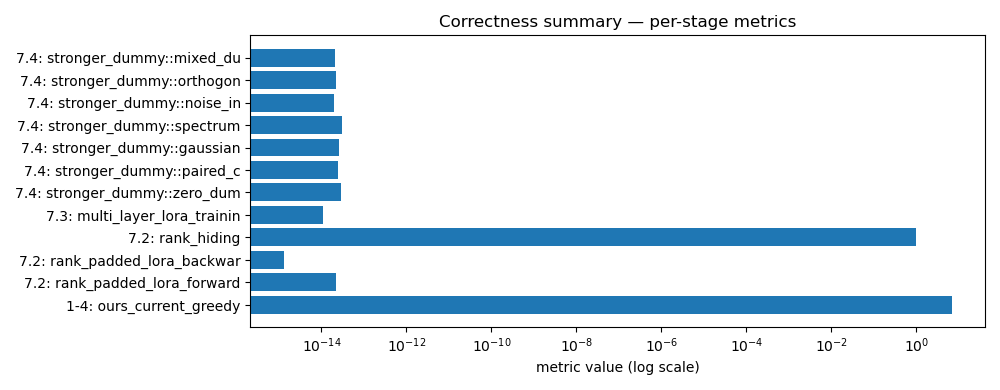
\includegraphics[width=0.88\linewidth]{figures/correctness_error_summary.png}
\caption{Per-component correctness error across the $19$ aggregated correctness rows of \Cref{tab:correctness-summary}. Empirical \texttt{allclose} equality on tested configurations only; we do not claim universal correctness.}
\label{fig:correctness-error-summary}
\end{figure}

\paragraph{Limitation.} Empirical equality on tested configurations only; modern-decoder model wrappers use synthetic or tiny-HF configurations, not production-scale Qwen, TinyLlama, or LLaMA.

\subsection{RQ2: Does the system support decoder-only generation with KV cache?}
\label{sec:eval:rq2}
\paragraph{Setup.} Greedy generation with KV cache append, per-step decode, RoPE rotation, and GQA. Evaluated for both GPT-2 (multi-head attention) and the modern decoder wrapper (GQA + RoPE).

\paragraph{Metric.} Sequence-level exact match against plain reference; per-step KV cache invariant.

\paragraph{Result.} Token-for-token exact match across the tested decode lengths; KV cache append invariant holds at every step.

\paragraph{Limitation.} Decoder-only with greedy sampling only. Top-$k$, top-$p$, beam search are implemented at the controller level but are not exercised in the security artifacts.

\subsection{RQ3: How much boundary-call and online-compute overhead does the method introduce?}
\label{sec:eval:rq3}
\paragraph{Setup.}
We compare \texttt{plain\_hf\_gpu}, \texttt{tslp\_trusted\_nonlinear\_baseline}, \texttt{ours\_current}, \texttt{ours\_compatible\_nonlinear\_islands}, \texttt{ours\_ideal\_gpu\_nonlinear}, and an \texttt{amulet\_style\_reference} cost-model baseline on tiny-GPT-2.

\paragraph{Metric.} Boundary-call count, trusted compute, GPU compute, preprocessing cost, projected wall-time, and (where measured) measured wall-time.

\paragraph{Result.} Boundary calls drop from $36$ for \texttt{ours\_current} to $16$ for \texttt{ours\_compatible\_nonlinear\_islands} and to $4$ for \texttt{ours\_ideal\_gpu\_nonlinear}. \Cref{fig:boundary-call-reduction} visualizes the reduction.

\begin{figure}[h]
\centering
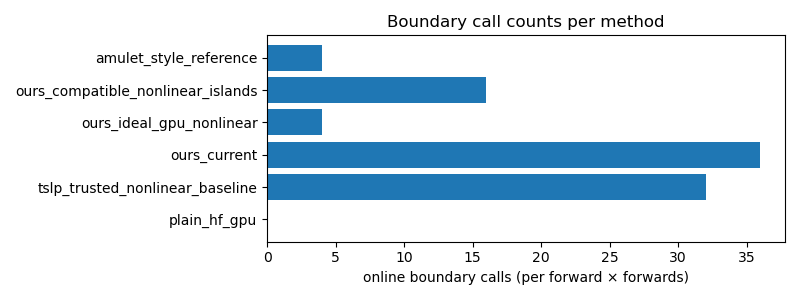
\includegraphics[width=0.82\linewidth]{figures/boundary_call_reduction.png}
\caption{Boundary-call reduction across method profiles. Workload-profile rows from \Cref{tab:workload-summary} on tiny-GPT-2 only; \texttt{wall\_time\_source = projected\_from\_op\_counts} for all but one row.}
\label{fig:boundary-call-reduction}
\end{figure}

\paragraph{Limitation.} Numbers are local-emulation projections on a tiny configuration ($n_\text{layer}=2$, $n_\text{embd}=2$, $n_\text{head}=2$); illustrative, not deployment numbers.

% Auto-generated by paper_artifact_consolidation
\begin{table}[h]
\centering
\small
\caption{Workload Summary}
\label{tab:workload\_summary}
\begin{tabular}{llllllllllll}
\toprule
method & architecture & integration\_level & boundary\_calls & trusted\_compute & gpu\_compute & preprocessing\_cost & online\_extra\_matmul\_count & measured\_wall\_time\_ms & projected\_wall\_time\_ms & wall\_time\_source & artifact\_path \\
\midrule
plain\_hf\_gpu & sshleifer/tiny-gpt2 & projected & 0 & 0 & 4434424 & 0 & 0 & 2.434716999414377 & 2.434716999414377 & measured & outputs/workload\_profile.json \\
tslp\_trusted\_nonlinear\_baseline & sshleifer/tiny-gpt2 & projected & 32 & 1110230 & 4429848 & 0 & 0 & None & 37.193893690611645 & projected\_from\_op\_counts & outputs/workload\_profile.json \\
ours\_current & sshleifer/tiny-gpt2 & projected & 36 & 1116310 & 4429848 & 403784 & 0 & 6.813033198704943 & 37.38195204023441 & measured & outputs/workload\_profile.json \\
ours\_ideal\_gpu\_nonlinear & sshleifer/tiny-gpt2 & projected & 4 & 1105654 & 4434424 & 403784 & 0 & None & 36.92668586094678 & projected\_from\_op\_counts & outputs/workload\_profile.json \\
ours\_compatible\_nonlinear\_islands & sshleifer/tiny-gpt2 & model\_level\_smoke & 16 & 1105830 & 4434424 & 403992 & 0 & None & 36.99217314509804 & projected\_from\_op\_counts & outputs/workload\_profile.json \\
amulet\_style\_reference & sshleifer/tiny-gpt2 & projected & 4 & 1105654 & 4434424 & 403784 & 0 & None & 36.92668586094678 & projected\_from\_op\_counts & outputs/workload\_profile.json \\
\bottomrule
\end{tabular}
\end{table}


\subsection{RQ4: How effective are the mitigation bundles against proxy attacks?}
\label{sec:eval:rq4}
\paragraph{Setup.} Proxy attackers (\Cref{sec:security}) against three mitigation configurations: \texttt{fresh\_perm\_only}, \texttt{fresh\_perm\_plus\_sandwich}, \texttt{fresh\_perm\_plus\_sandwich\_plus\_pad}.

\paragraph{Metric.} Per-attacker accuracy and linkability AUC; consolidated into a risk-level matrix (\Cref{fig:security-risk-matrix,tab:security-proxy-summary}).

\paragraph{Result.} The full bundle reduces every adaptive-inverter accuracy to ``close to random chance'' status. Specific rows: black-box query attacker \texttt{low} distinguishability; ridge/MLP/signature/Sinkhorn attackers \texttt{needs\_more\_evaluation}; timing classifier under \texttt{proxy\_equalized} is \texttt{low}.

\paragraph{Limitation.} Proxy attackers only; not a formal-security claim. \texttt{high}-risk rows (gradient rank inference, stronger-dummy spectral inference) are reported and not re-classified.

\subsection{RQ5: Does the LoRA private training path preserve correctness?}
\label{sec:eval:rq5}
\paragraph{Setup.} Synthetic single-linear and synthetic multi-layer LoRA training: masked forward, masked backward, rank-padded forward $+$ backward, multi-layer training step across $2$ layers and $14$ modules, and five stronger dummy distributions.

\paragraph{Metric.} $\max$-loss-diff, $\max$-grad-error, $\max$-update-error, \texttt{allclose}.

\paragraph{Result.} Across all $11$ LoRA-side rows (\Cref{tab:lora-training-summary}), the masked path matches the plain reference to float64 precision ($\max$-grad-$A$ error $\in [10^{-15}, 2\times 10^{-15}]$, $\max$-update-error $\in [10^{-17}, 10^{-16}]$). \Cref{fig:lora-training-errors} plots the errors.

\begin{figure}[h]
\centering
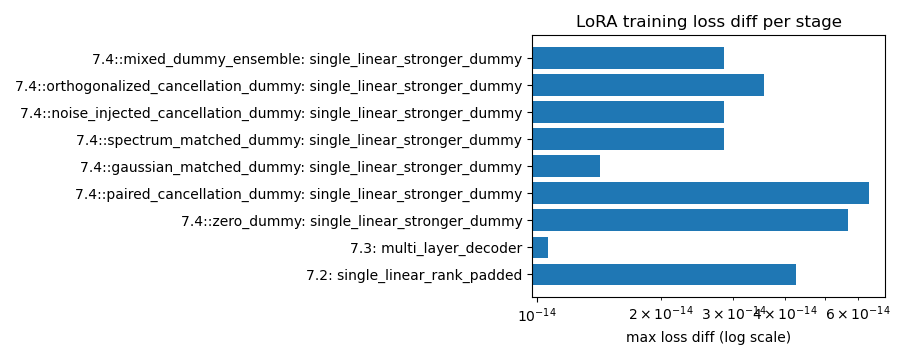
\includegraphics[width=0.82\linewidth]{figures/lora_training_errors.png}
\caption{LoRA training errors across Stages 7.0--7.4 (synthetic tiles). Empirical \texttt{allclose} matches to float64 precision; no production fine-tune of Qwen, TinyLlama, or LLaMA is run.}
\label{fig:lora-training-errors}
\end{figure}

\paragraph{Limitation.} Synthetic tiles only. Loss and optimizer remain trusted-side. PEFT~\cite{peft2022}, DeepSpeed~\cite{rasley2020deepspeed}, vLLM~\cite{kwon2023vllm}, FlashAttention~\cite{dao2022flashattention} are not integrated.

% Auto-generated by paper_artifact_consolidation
\begin{table}[h]
\centering
\small
\caption{LoRA Training Summary}
\label{tab:lora\_training\_summary}
\begin{tabular}{lllllllllllll}
\toprule
stage & training\_scope & num\_layers & num\_lora\_modules & true\_rank & padded\_rank & optimizer & loss\_diff & grad\_error & update\_error & rank\_hidden\_from\_shape & risk\_level & artifact\_path \\
\midrule
7.0 & single\_linear & 1 & 1 & 4 & 4 & sgd & None & None & None & False & needs\_more\_evaluation & outputs/lora\_training\_experiments.json \\
7.1 & single\_linear\_masked\_backward & 1 & 1 & 4 & 4 & sgd & None & None & None & False & needs\_more\_evaluation & outputs/lora\_backward\_experiments.json \\
7.2 & single\_linear\_rank\_padded & 1 & 1 & 4 & 8 & sgd & 4.263256414560601e-14 & 1.3062467774105357e-15 & 1.1102230246251565e-16 & True & needs\_more\_evaluation & outputs/lora\_rank\_padding\_experiments.json \\
7.3 & multi\_layer\_decoder & 2 & 14 & 4 & 8 & sgd & 1.0658141036401503e-14 & 1.8446615762668372e-15 & 5.551115123125783e-17 & True & needs\_more\_evaluation & outputs/multilayer\_lora\_training\_experiments.json \\
7.4::zero\_dummy & single\_linear\_stronger\_dummy & 1 & 1 & 4 & 16 & sgd & 5.684341886080802e-14 & 1.1102230246251565e-16 & 2.7755575615628914e-17 & True & needs\_more\_evaluation & outputs/lora\_stronger\_dummy\_experiments.json \\
7.4::paired\_cancellation\_dummy & single\_linear\_stronger\_dummy & 1 & 1 & 4 & 16 & sgd & 6.394884621840902e-14 & 2.5283594662361963e-15 & 5.551115123125783e-17 & True & needs\_more\_evaluation & outputs/lora\_stronger\_dummy\_experiments.json \\
7.4::gaussian\_matched\_dummy & single\_linear\_stronger\_dummy & 1 & 1 & 4 & 16 & sgd & 1.4210854715202004e-14 & 1.1102230246251565e-16 & 5.551115123125783e-17 & True & needs\_more\_evaluation & outputs/lora\_stronger\_dummy\_experiments.json \\
7.4::spectrum\_matched\_dummy & single\_linear\_stronger\_dummy & 1 & 1 & 4 & 16 & sgd & 2.842170943040401e-14 & 1.942890293094024e-16 & 5.551115123125783e-17 & True & needs\_more\_evaluation & outputs/lora\_stronger\_dummy\_experiments.json \\
7.4::noise\_injected\_cancellation\_dummy & single\_linear\_stronger\_dummy & 1 & 1 & 4 & 16 & sgd & 2.842170943040401e-14 & 2.5431046157819992e-15 & 5.551115123125783e-17 & True & needs\_more\_evaluation & outputs/lora\_stronger\_dummy\_experiments.json \\
7.4::orthogonalized\_cancellation\_dummy & single\_linear\_stronger\_dummy & 1 & 1 & 4 & 16 & sgd & 3.552713678800501e-14 & 7.528699885739343e-16 & 5.551115123125783e-17 & True & needs\_more\_evaluation & outputs/lora\_stronger\_dummy\_experiments.json \\
7.4::mixed\_dummy\_ensemble & single\_linear\_stronger\_dummy & 1 & 1 & 4 & 16 & sgd & 2.842170943040401e-14 & 7.754213937616328e-16 & 5.551115123125783e-17 & True & needs\_more\_evaluation & outputs/lora\_stronger\_dummy\_experiments.json \\
\bottomrule
\end{tabular}
\end{table}


\subsection{RQ6: How much leakage remains from rank, timing, and metadata?}
\label{sec:eval:rq6}
\paragraph{Setup.} Spectral-rank-inference, gradient-rank-inference, dummy-strategy classifier, cross-layer linkage, and cost-model training-timing classifier evaluated across Stages 7.2--7.4.

\paragraph{Result.}
Spectral rank inference under \texttt{paired\_cancellation\_dummy}: \texttt{needs\_more\_evaluation}. Gradient rank inference: \texttt{high}. Stronger-dummy spectral inference worst-case: \texttt{high}. Stronger-dummy gradient inference worst-case: \texttt{high}. Dummy-strategy classifier accuracy: $0.476$ vs chance $0.143$, risk \texttt{medium}. Cross-layer linkage with fresh masks per module $+$ paired cancellation: \texttt{low}. Training-step cost-model timing under \texttt{proxy\_equalized}: $0.5124$, risk \texttt{low}. \Cref{fig:rank-inference-risk,fig:timing-proxy-before-after} visualize these.

\begin{figure}[h]
\centering
\begin{subfigure}{0.49\linewidth}
  \centering
  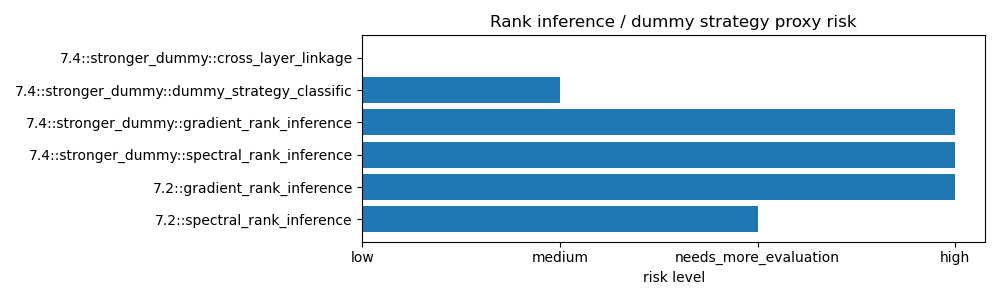
\includegraphics[width=\linewidth]{figures/rank_inference_risk.png}
  \caption{Rank-inference risk across detectors and dummy strategies. \texttt{high} cells are reported faithfully and not re-classified.}
  \label{fig:rank-inference-risk}
\end{subfigure}
\hfill
\begin{subfigure}{0.49\linewidth}
  \centering
  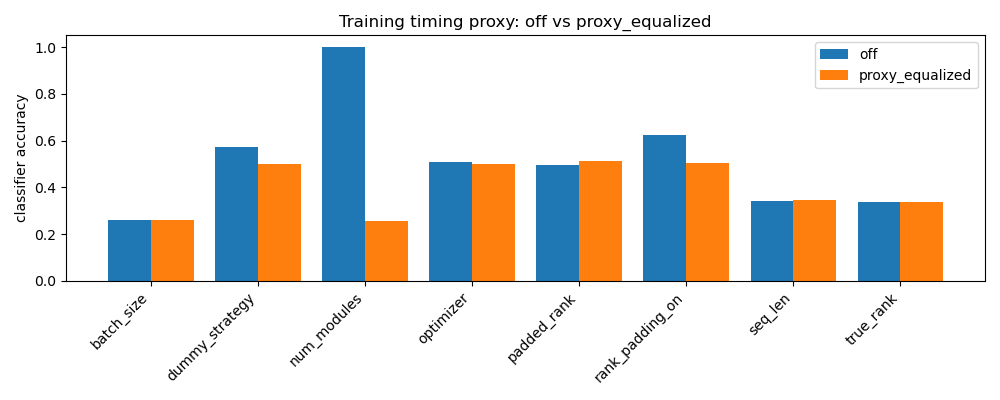
\includegraphics[width=\linewidth]{figures/timing_proxy_before_after.png}
  \caption{Cost-model timing classifier before vs.\ after \texttt{proxy\_equalized}. Proxy only; not real wall-time and not a hardware side-channel evaluation.}
  \label{fig:timing-proxy-before-after}
\end{subfigure}
\caption{Rank-inference and timing-proxy results across Stages 7.2--7.4.}
\label{fig:rank-and-timing}
\end{figure}

\paragraph{Limitation.} Spectral- and gradient-inference \texttt{high}-risk rows are honest open problems; they motivate heterogeneous padded rank and stronger spectral hardening as future work.

\subsection{RQ7: What is the measured local runtime overhead?}
\label{sec:eval:rq7}
\paragraph{Setup.} \texttt{time.perf\_counter} benchmarks of six primitives (synthetic baseline, plain LoRA forward, masked LoRA forward/backward, rank-padded forward, multi-layer training step) plus an opt-in modern-decoder-model-wrapper benchmark (skipped by default with reason \texttt{include\_modern\_decoder\_wrapper=False}). $\text{num\_warmup}=2$, $\text{num\_repeats}=5$, $\text{device}=\text{cpu}$, $\text{dtype}=\text{float64}$, $\text{wall\_time\_source}=\text{measured\_local\_emulation}$.

\paragraph{Result.} Mean times (illustrative): \texttt{plain\_synthetic\_linear} $0.002$\,ms, \texttt{plain\_lora\_forward} $0.008$\,ms, \texttt{masked\_lora\_forward} $0.263$\,ms, \texttt{masked\_lora\_backward} $0.118$\,ms, \texttt{rank\_padded\_lora\_forward} $0.270$\,ms, \texttt{multi\_layer\_lora\_training\_step} $4.684$\,ms. \Cref{fig:measured-runtime-summary} plots the distribution.

\begin{figure}[h]
\centering
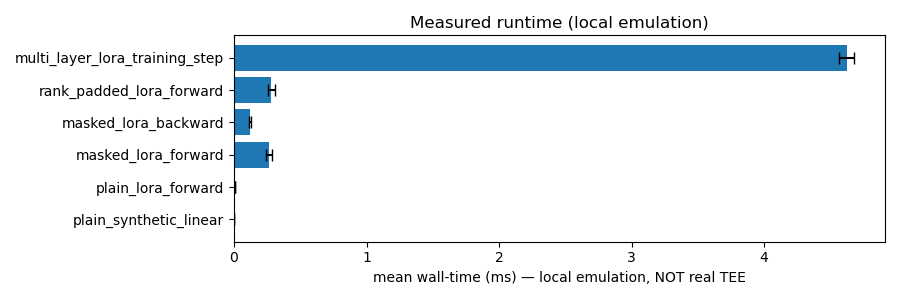
\includegraphics[width=0.82\linewidth]{figures/measured_runtime_summary.png}
\caption{\textbf{Local-emulation runtime per primitive (this is \emph{not} real TEE wall-time).} $\text{num\_warmup}=2$, $\text{num\_repeats}=5$, $\text{device}=\text{cpu}$, $\text{dtype}=\text{float64}$, $\text{wall\_time\_source}=\text{measured\_local\_emulation}$.}
\label{fig:measured-runtime-summary}
\end{figure}

\paragraph{Limitation. This is local runtime emulation, not real TEE wall-time.} No real sleep, no real runtime gating; \texttt{time.perf\_counter} only. Workload tiles are small for test stability; absolute numbers are illustrative.

% Auto-generated by measured_runtime_evaluation
\begin{table}[h]
\centering
\small
\caption{Measured runtime (local emulation, NOT real TEE wall-time).}
\label{tab:measured_runtime}
\begin{tabular}{llllllllllllll}
\toprule
component & variant & num\_warmup & num\_repeats & mean\_ms & median\_ms & std\_ms & min\_ms & max\_ms & device & dtype & wall\_time\_source & skipped\_with\_reason & notes \\
\midrule
plain\_synthetic\_linear & X W & 2 & 5 & 0.0017916012438945472 & 0.0017080019460991025 & 0.00025515530856451467 & 0.0015420009731315076 & 0.002082997525576502 & cpu & float64 & measured\_local\_emulation & None & Synthetic baseline; no obfuscation. \\
plain\_lora\_forward & plain\_rank\_r & 2 & 5 & 0.007958199421409518 & 0.007791000825818628 & 0.0006766130077735035 & 0.007333001121878624 & 0.00904199987417087 & cpu & float64 & measured\_local\_emulation & None & Plain rank-r LoRA forward; no masking. \\
masked\_lora\_forward & fresh\_masks\_fresh\_u\_with\_pad & 2 & 5 & 0.2471915984642692 & 0.24466699687764049 & 0.015932198492687927 & 0.22724999871570617 & 0.27033299556933343 & cpu & float64 & measured\_local\_emulation & None & Stage 7.0 run\_masked\_lora\_linear forward. \\
masked\_lora\_backward & fresh\_masks\_fresh\_u\_with\_pad & 2 & 5 & 0.11866640124935657 & 0.11804100358858705 & 0.0036911838356562545 & 0.11600000289035961 & 0.1249999986612238 & cpu & float64 & measured\_local\_emulation & None & Stage 7.1 run\_masked\_lora\_backward. \\
rank\_padded\_lora\_forward & paired\_cancellation\_dummy & 2 & 5 & 0.27414139913162217 & 0.2795830005197786 & 0.01261367039715004 & 0.2536250030971132 & 0.28458299493649974 & cpu & float64 & measured\_local\_emulation & None & Stage 7.2 rank-padded masked forward. \\
multi\_layer\_lora\_training\_step & synthetic\_tile & 2 & 5 & 4.635358400992118 & 4.605207999702543 & 0.07070563046014282 & 4.554750004899688 & 4.732041998067871 & cpu & float64 & measured\_local\_emulation & None & Stage 7.3 run\_multilayer\_lora\_training (one training step). \\
modern\_decoder\_model\_wrapper & opt\_in\_only & 2 & 5 & None & None & None & None & None & cpu & float64 & measured\_local\_emulation & modern\_decoder\_wrapper is opt-in (include\_modern\_decoder\_... & Opt-in benchmark; pytest defaults stay synthetic. \\
\bottomrule
\end{tabular}
\end{table}


\subsection{RQ8: Does the method remain correct on task-like toy workloads?}
\label{sec:eval:rq8}
\paragraph{Setup.} Three deterministic synthetic toy tasks exercise plain vs. masked execution on task-like inputs rather than random tensors: \texttt{token\_parity\_classification} (label = $\sum \text{input\_ids} \bmod 2$), \texttt{first\_last\_token\_relation} (label = $\mathbb{1}[\text{first\_token} < \text{last\_token}]$), and \texttt{next\_token\_toy\_lm} (target = a deterministic function of the previous tokens). The tiny LoRA-augmented decoder stack is shared across paths; we run a short SGD loop (analytic backward on the plain reference, trusted-side update) and compare per-step plain vs.\ masked loss, accuracy, logits, and token-match.

\paragraph{Metric.} \texttt{loss\_diff}, \texttt{accuracy\_diff}, \texttt{logits\_max\_abs\_error}, \texttt{token\_match\_rate}, \texttt{allclose}.

\paragraph{Result.} Across all three tasks, the masked path reproduces the plain reference to float64 round-off (\texttt{loss\_diff} $\leq 10^{-15}$, \texttt{accuracy\_diff} $= 0$, \texttt{token\_match\_rate} $= 1$, \texttt{allclose} $= \text{True}$). See \Cref{tab:toy-task-summary}.

\paragraph{Limitation.} Deterministic synthetic tasks; no external dataset, no tokenizer, not a real Qwen / TinyLlama / LLaMA fine-tune.

% Auto-generated by paper_artifact_consolidation
\begin{table}[h]
\centering
\small
\caption{Toy Task Summary (CPU only)}
\label{tab:toy\_task\_summary}
\begin{tabular}{lllllllllllll}
\toprule
task\_name & num\_samples & num\_train\_steps & train\_loss\_plain & train\_loss\_masked & loss\_diff & accuracy\_plain & accuracy\_masked & accuracy\_diff & logits\_max\_abs\_error & token\_match\_rate & allclose & runtime\_ms \\
\midrule
token\_parity\_classification & 128 & 20 & 0.6901150550410321 & 0.6901150550410321 & 0.0 & 0.5390625 & 0.5390625 & 0.0 & 9.992007221626409e-16 & 1.0 & True & 23.32412500004466 \\
first\_last\_token\_relation & 128 & 20 & 0.688203308355396 & 0.6882033083553959 & 1.1102230246251565e-16 & 0.53125 & 0.53125 & 0.0 & 7.042977312465837e-16 & 1.0 & True & 12.599417000046742 \\
next\_token\_toy\_lm & 128 & 20 & 4.8663778912838485 & 4.866377891283849 & 8.881784197001252e-16 & 0.015625 & 0.015625 & 0.0 & 3.3931191190106347e-15 & 1.0 & True & 13.031958000055965 \\
\bottomrule
\end{tabular}
\end{table}


\subsection{RQ9: How do baselines compare under the same CPU local-emulation setting?}
\label{sec:eval:rq9}
\paragraph{Setup.} Ten variants on a single CPU synthetic tile: \texttt{plain\_cpu}, \texttt{trusted\_nonlinear\_partition}, \texttt{fixed\_permutation\_only}, \texttt{fresh\_perm\_only}, \texttt{full\_mitigation\_bundle}, \texttt{full\_bundle\_masked\_boundary}, \texttt{full\_bundle\_masked\_boundary\_constant\_time\_proxy}, \texttt{lora\_plain}, \texttt{lora\_masked\_forward\_backward}, and \texttt{lora\_rank\_padded}.

\paragraph{Metric.} \texttt{correctness\_error}, \texttt{token\_match\_rate}, \texttt{loss\_diff}, structurally-derived \texttt{boundary\_calls}, local CPU \texttt{local\_runtime\_ms}, proxy-derived \texttt{proxy\_risk\_level}.

\paragraph{Result.} Each masked variant matches the plain reference to float64 round-off; risk levels span \texttt{high} (\texttt{plain\_cpu}, \texttt{fixed\_permutation\_only}, \texttt{lora\_plain}), \texttt{medium} (\texttt{fresh\_perm\_only}), \texttt{needs\_more\_evaluation} (full bundle and masked variants), and \texttt{low} (full bundle + \texttt{proxy\_equalized}). See \Cref{tab:baseline-comparison-summary}.

\paragraph{Limitation.} Risk levels are proxy-derived from the existing Stage~5--7 security proxy summary, not formal security guarantees; boundary-call counts are structurally derived from the mitigation configuration, not measured kernel launches.

% Auto-generated by paper_artifact_consolidation
\begin{table}[h]
\centering
\small
\caption{Baseline Comparison Summary (CPU only)}
\label{tab:baseline\_comparison\_summary}
\begin{tabular}{llllllllll}
\toprule
variant & kind & correctness\_error & token\_match\_rate & loss\_diff & boundary\_calls & online\_extra\_matmul\_count & local\_runtime\_ms & proxy\_risk\_level & supported\_claim\_type \\
\midrule
plain\_cpu & inference & 0.0 & 1.0 & 0.0 & 0 & 0 & 0.008558599984098691 & high & baseline \\
trusted\_nonlinear\_partition & inference & 5.620504062164855e-16 & 1.0 & 6.938893903907228e-18 & 32 & 0 & 0.14833339996584982 & needs\_more\_evaluation & tee\_partition\_baseline \\
fixed\_permutation\_only & inference & 2.942091015256665e-15 & 1.0 & 4.163336342344337e-17 & 4 & 0 & 0.16578320000917302 & high & risk\_baseline \\
fresh\_perm\_only & inference & 3.400058012914542e-15 & 1.0 & 1.3877787807814457e-17 & 4 & 0 & 0.16774159998931282 & medium & partial\_mitigation \\
full\_mitigation\_bundle & inference & 3.5041414214731503e-15 & 1.0 & 0.0 & 16 & 0 & 0.15381700004581944 & needs\_more\_evaluation & proxy\_supported\_main \\
full\_bundle\_masked\_boundary & inference & 2.8449465006019636e-15 & 1.0 & 0.0 & 4 & 0 & 0.14143339999463933 & needs\_more\_evaluation & proxy\_supported\_ablation \\
full\_bundle\_masked\_boundary\_constant\_time\_proxy & inference & 2.858824288409778e-15 & 1.0 & 6.938893903907228e-18 & 4 & 0 & 0.1406919999681122 & low & proxy\_supported\_timing \\
lora\_plain & lora & 0.0 & 1.0 & 0.0 & 0 & 0 & 0.008316399998875568 & high & lora\_baseline \\
lora\_masked\_forward\_backward & lora & 2.6367796834847468e-15 & 1.0 & 0.0 & 2 & 0 & 0.14179160002640856 & needs\_more\_evaluation & proxy\_supported\_lora \\
lora\_rank\_padded & lora & 1.6833756610878936e-14 & 1.0 & 4.85722573273506e-17 & 2 & 0 & 0.191816799906519 & needs\_more\_evaluation & proxy\_supported\_rank \\
\bottomrule
\end{tabular}
\end{table}


\subsection{RQ10: Which mitigation components are necessary?}
\label{sec:eval:rq10}
\paragraph{Setup.} For each mitigation axis (boundary pad, permutation freshness, dense sandwich, inter-block boundary, constant-time decode proxy, rank padding, dummy strategy) we toggle settings and record correctness, proxy risk level, runtime overhead, and an \texttt{interpretation} tag.

\paragraph{Result.} Correctness is preserved by construction across both settings of every axis -- each axis is an algebraic identity (Theorems~1--9). The boundary pad, fresh permutation, dense sandwich, rank padding, and stronger dummy strategy are tagged \texttt{security\_critical}; the cost-model constant-time decode proxy is \texttt{metadata\_timing}; the inter-block masked boundary is \texttt{experimental\_optin}. See \Cref{tab:ablation-summary}.

\paragraph{Limitation.} No axis is \emph{correctness}-critical, so the ablation matrix does not change \texttt{allclose}; the table is informative about \emph{proxy} security and \emph{runtime} only.

% Auto-generated by paper_artifact_consolidation
\begin{table}[h]
\centering
\small
\caption{Mitigation Ablation Summary (CPU only)}
\label{tab:ablation\_summary}
\begin{tabular}{llllllll}
\toprule
component & setting & correctness\_preserved & max\_abs\_error & proxy\_attack\_metric & risk\_level & runtime\_overhead\_ms & interpretation \\
\midrule
boundary\_pad & off & True & 9.43689570931383e-16 & activation\_recovery\_proxy & high & 0.12207825000842831 & security\_critical \\
boundary\_pad & on & True & 3.649858193455202e-15 & activation\_recovery\_proxy & needs\_more\_evaluation & 0.1433515000073271 & security\_critical \\
permutation\_freshness & fixed & True & 4.135580766728708e-15 & linkability\_auc & high & 0.05202350001098921 & security\_critical \\
permutation\_freshness & fresh & True & 4.6074255521944e-15 & linkability\_auc & needs\_more\_evaluation & 0.1516848750071631 & security\_critical \\
dense\_sandwich & off & True & 7.771561172376096e-16 & permutation\_recovery\_proxy & high & 0.13928262501394784 & security\_critical \\
dense\_sandwich & on & True & 4.433953204596719e-15 & permutation\_recovery\_proxy & needs\_more\_evaluation & 0.1555664062635742 & security\_critical \\
inter\_block\_boundary & plain\_boundary & True & 0.0 & inter\_block\_linkability\_proxy & needs\_more\_evaluation & 0.0 & security\_critical \\
inter\_block\_boundary & masked\_boundary\_experimental & True & 0.0 & inter\_block\_linkability\_proxy & needs\_more\_evaluation & 0.0 & experimental\_optin \\
constant\_time\_decode\_proxy & off & True & 0.0 & cost\_model\_timing\_classifier\_accuracy & medium & 0.0 & metadata\_timing \\
constant\_time\_decode\_proxy & proxy\_equalized & True & 0.0 & cost\_model\_timing\_classifier\_accuracy & low & 0.0 & metadata\_timing \\
rank\_padding & off & True & 3.941291737419306e-15 & spectral\_rank\_inference\_proxy & high & 0.15531509372834762 & security\_critical \\
rank\_padding & on & True & 3.577693696854567e-14 & spectral\_rank\_inference\_proxy & needs\_more\_evaluation & 0.18661728127256083 & security\_critical \\
dummy\_strategy & zero\_dummy & True & 4.538036613155327e-15 & spectral\_rank\_inference\_proxy & high & 0.1703737500164948 & security\_critical \\
dummy\_strategy & paired\_cancellation\_dummy & True & 4.230643613212237e-14 & spectral\_rank\_inference\_proxy & needs\_more\_evaluation & 0.18259381248242335 & security\_critical \\
dummy\_strategy & spectrum\_matched\_dummy & True & 3.5110803153770576e-15 & spectral\_rank\_inference\_proxy & needs\_more\_evaluation & 0.24155587500729325 & security\_critical \\
dummy\_strategy & mixed\_dummy\_ensemble & True & 3.2612801348363973e-14 & spectral\_rank\_inference\_proxy & needs\_more\_evaluation & 0.25806765623315187 & security\_critical \\
\bottomrule
\end{tabular}
\end{table}


\subsection{RQ11: Are correctness and proxy trends stable across seeds and shapes?}
\label{sec:eval:rq11}
\paragraph{Setup.} Sweep \texttt{seeds} $\in \{2021, 2022, 2023, 2024, 2025\}$, \texttt{batch\_sizes} $\in \{1, 2, 4, 8\}$, \texttt{seq\_lens} $\in \{4, 8, 16\}$, \texttt{hidden\_sizes} $\in \{16, 32, 64\}$, \texttt{true\_ranks} $\in \{2, 4\}$, \texttt{padded\_ranks} $\in \{8, 16\}$ across seven experiments: modern decoder synthetic forward, KV cache append, nonlinear island, LoRA forward, LoRA backward, rank-padded LoRA, multi-layer LoRA.

\paragraph{Result.} \texttt{allclose\_rate} = 1.0 for every experiment in the swept space; \texttt{max\_error\_p95} stays at the float64 round-off level ($10^{-16}$ to $10^{-14}$); \texttt{failure\_count} = 0 except for explicitly-skipped configurations (e.g., \texttt{rank > hidden}). See \Cref{tab:stability-summary}.

\paragraph{Limitation.} Stability is measured by the spread of float64 round-off across seeds and shapes; it is \emph{not} a security metric.

% Auto-generated by paper_artifact_consolidation
\begin{table}[h]
\centering
\small
\caption{Robustness/Stability Summary (CPU only)}
\label{tab:stability\_summary}
\begin{tabular}{llllllll}
\toprule
experiment & trials & allclose\_rate & max\_error\_p95 & max\_error\_max & runtime\_mean & runtime\_std & failure\_count \\
\midrule
modern\_decoder\_synthetic\_forward & 720 & 1.0 & 1.942890293094024e-16 & 3.0531133177191805e-16 & 0.09044245416968504 & 0.12069696616987177 & 0 \\
kv\_cache\_append & 720 & 1.0 & 2.220446049250313e-15 & 2.6645352591003757e-15 & 0.02133661666271615 & 0.011569293885244582 & 0 \\
nonlinear\_island & 720 & 1.0 & 0.0 & 0.0 & 0.020318999992873107 & 0.01990172099099236 & 0 \\
lora\_forward & 720 & 1.0 & 4.055783486833775e-15 & 5.3013149425851225e-15 & 0.2250337722222816 & 0.11779534355212642 & 0 \\
lora\_backward & 720 & 1.0 & 4.529709940470639e-14 & 8.304468224196171e-14 & 0.35323947638580144 & 0.165506555278635 & 0 \\
rank\_padded\_lora & 720 & 1.0 & 7.732703366514215e-14 & 1.5466794511809212e-13 & 0.22593616528562657 & 0.10856064283419462 & 0 \\
multilayer\_lora & 720 & 1.0 & 5.717648576819556e-15 & 6.147859998861804e-15 & 0.44706556666685376 & 0.22340250656771193 & 0 \\
\bottomrule
\end{tabular}
\end{table}


\subsection{RQ12: What CPU-only runtime overhead is observed across components?}
\label{sec:eval:rq12}
\paragraph{Setup.} Twelve components (\texttt{linear\_masked\_forward}, \texttt{nonlinear\_island\_forward}, \texttt{modern\_decoder\_full\_forward}, \texttt{modern\_decoder\_prefill}, \texttt{modern\_decoder\_decode\_step}, \texttt{modern\_decoder\_greedy\_generation}, \texttt{lora\_forward}, \texttt{lora\_backward}, \texttt{lora\_rank\_padding}, \texttt{multilayer\_lora\_training\_step}, \texttt{stronger\_dummy\_generation}, \texttt{paper\_toy\_task\_train\_step}) swept over \texttt{(batch\_size, seq\_len, hidden\_size)} $\in \{1,4\} \times \{8, 16\} \times \{32, 64\}$. $\text{num\_warmup}=3$, $\text{num\_repeats}=20$, $\text{dtype}=\text{float64}$, $\text{device}=\text{cpu}$.

\paragraph{Result.} Each row records \texttt{mean\_ms}, \texttt{median\_ms}, \texttt{std\_ms}, \texttt{min\_ms}, \texttt{max\_ms}. See \Cref{tab:cpu-runtime-completion}.

\paragraph{Limitation.} \textbf{This is CPU local trusted-runtime emulation, NOT real TEE wall-time and NOT GPU throughput.} No \texttt{time.sleep}; modern-decoder rows use synthetic stand-ins; no PEFT / DeepSpeed / vLLM / FlashAttention integration.

\input{tables/cpu_runtime_completion.tex}

\subsection{Cross-cutting observations}
\label{sec:eval:summary}
The full mitigation bundle is \emph{required}; partial bundles leak more under the same attackers. Stronger dummy distributions improve cross-layer linkage to \texttt{low} but do not improve worst-case rank inference. The toy-task and stability sweeps confirm the algebraic identities of Theorems~1--9 hold on task-like inputs and across the swept seed/shape space; the baseline comparison and ablation rows expose the structural trade-offs between mitigation knobs. Local-emulation runtime is a coarse signal whose primary use is to confirm that no trusted-side primitive is catastrophically slow at this scale; it is \emph{not} a deployment latency claim, not real TEE wall-time, and not GPU throughput.
